\newcommand\tab[1][1cm]{\hspace*{#1}}
\chapter[Biochémia]{Biochémia}
\label{biochemia} % id kapitoly pre prikaz ref

%1
\section{Chémia ako logický základ biologického fenoménu}
Status: DONE
Source: Prezentácia 1
\\
\subsection*{Základné vlastnosti živých systémov}
Zložité a organizované\\
Bio štruktúry majú funkčný význam\\
Aktívne zapojené do premien energie\\
Schopnosť replikácie\\
Chemický základ
\subsection*{Biomolekuly}
HOCN -- schopnosť vytvárať kovalentné väzby cez e\textsuperscript{-} páry $\rightarrow$ rôzne štruktúry
\subsection*{Vlastnosti biomolekúl}
Štruktúrna polarita (napr. 5' $\rightarrow$ 3')\\
Informatívnosť (napr. DNA, polypeptidy)\\
Trojrozmerná štruktúra\\
\subsection*{Vlastnosti vody}
Vysoká hodnota teploty topenia a varu, výparného tepla, povrchového napätia\\
Polarita $\leftarrow$ Lomená štruktúra\\
Tvorba vodíkových väzieb\\
Solvatačné vlastnosti\\
\tab Polárne látky $\rightarrow$ vodíkové väzby\\
\tab Nepolárne $\rightarrow$ hydrofóbne interakcie
\subsection*{Typy a význam slabých interakcií v biologických štruktúrach}
Slabé interakcie udržujú 3D štruktúru a určujú interakcie\\
\tab Napr. biomolekulárne rozpoznávanie\\
\tab Obmedzené vhodné enviromentálne podmienky\\
Van der Waalsove\\
Vodíkové\\
Iónové\\
Hydrofóbne
\subsection*{Hydrofóbne interakcie}
Disperzia lipidov $\rightarrow$ usporiadavajú okolitú H2O\\
Lipidy sa zoskupujú $\rightarrow$ entropia systému rastie, výhodnejší stav\\
Micely $\rightarrow$ hydrofóbne konce idú dnu, entropia systému vyššia\\

%2
\section{Aminokyseliny a proteíny}

Status: DONE
Source: Prezentácia 1
\\
\subsection*{Všeobecný vzorec AK}
\includegraphics[width=0.25\textwidth, page=35]{materials/Biochemia/Prezentacie_Biochemia/01_Uvod_AK_Proteiny.pdf}
\subsection*{Klasifikácia AK}
D, L izoméria\\
rozdelenie na základe chem vlastností side chain\\
\tab náboj\\
\tab schopnosť viazať H\\
\tab Kyslá/zásaditá\\
Nepolárne -- hydrofóbne\\
Polárne -- hydrofilné
\subsection*{vzorce AK}
\includegraphics[width=0.5\textwidth, page=37]{materials/Biochemia/Prezentacie_Biochemia/01_Uvod_AK_Proteiny.pdf}
\includegraphics[width=0.5\textwidth, page=38]{materials/Biochemia/Prezentacie_Biochemia/01_Uvod_AK_Proteiny.pdf}
\\
Tvorba disulfidovej väzby

\includegraphics[width=0.5\textwidth, page=39]{materials/Biochemia/Prezentacie_Biochemia/01_Uvod_AK_Proteiny.pdf}
\\
\subsection*{optická aktivita}
Schopnosť otáčať rovinu polarizovaného svetla -- napr. Vlnenie fotónu ide zhora dole $\rightarrow$ zľava doprava\\
Všetky AK okrem glycínu\\
L a D aminokyseliny \\

\includegraphics[width=0.5\textwidth, page=44]{materials/Biochemia/Prezentacie_Biochemia/01_Uvod_AK_Proteiny.pdf}
\\
\subsection*{spektroskopické vlastnosti AK}
Absorbujú v infrač. oblasti\\
Trp a tyr, menej Phe v UV\\
Absorbcia pri 280nm sa používa pri detekcii proteínov\\
\\
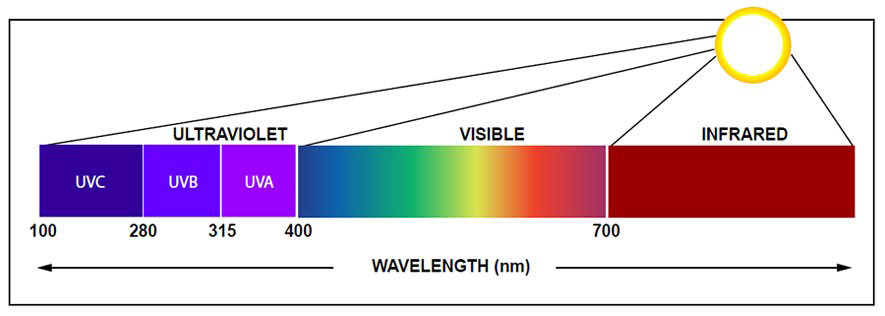
\includegraphics[width=0.5\textwidth]{images/wavelength}
\\
\subsection*{acidobázické vlastnosti AK}
Pri nízkom pH je veľa H+, AK stráca čiastočne negatívny náboj a ostane s kladným. \\
Pri vysokom pH je veľa OH-- $\rightarrow$ bude mať záporný náboj\\
\subsection*{Zwitterióny, amfotérny charakter AK, }
Pri neutrálnom pH má oba náboje $\rightarrow$ Zwitterión/Amfión\\
Vie reagovať s kys. aj zásadami\\
\subsection*{izoelektrický bod}
izoelektrický bod: pH, keď sa AK mení z -- na 0 alebo z + na 0.\\
\tab pI = (pKA kyslého + pKA zásaditého)/2. Obyčajne 9 a 2\\
\tab pI = average of pKAs of functional groups
\subsection*{štruktúra a vlastnosti peptidovej väzby}

\includegraphics[width=0.5\textwidth, page=46]{materials/Biochemia/Prezentacie_Biochemia/01_Uvod_AK_Proteiny.pdf}
\\
Odchádza/prichádza H2O\\
N\textsuperscript{+}, O\textsuperscript{-}
medzi jednoduchou a dvojitou\\
trans\\
6 atómov v rovine -- planárne usporiadanie
\subsection*{Trojrozmerná štruktúra proteínov}
primárna, sekundárna ($\alpha$--helix, $\beta$--skladaný list, $\beta$--otáčka), terciárna, kvartérna, 
väzby (interakcie) a funkčné skupiny uplatňujúce sa pri jednotlivých štruktúrach\\
\\
Primárna\\
\tab poradie AK, kovalentné peptidové väzby\\
Sekundárna\\
\tab ako sa skladajú na seba, (základná štruktúra, nie zvyšky), vodíkové väzby medzi CO a NH\\
\tab $\alpha$--helix (pravotočivý)\\
\tab \tab Väzba o 4 zvyšky dopredu\\
\tab $\beta$--skladaný list\\
\tab \tab paralelný, antiparalelný\\
\tab \tab Úplne rozvinutý reťazec\\
\tab \tab Väzby aj medzi rozdielnymi reťazcami\\
\tab $\beta$--otáčka\\
\tab \tab Zmena smeru peptidového reťazcu\\
\tab \tab Väzba o 3 zvyšky ďalej\\
\tab \tab prolín, glycín\\
Terciárna\\
\tab Priestorová štruktúra, interakcie vzdialených skupín, ako sa folds skladajú na seba, vodíkové väzby, Van der Waals, hydrofóbny obal, disulfidový mostík medzi bočnými reťazcami\\
\tab Daná primárnou štruktúrou\\
kvartérna\\
\tab medzi rôznymi polypeptidmi\\
\tab podjednotky sa skladajú do mérov -- diméry, tetraméry, multiméry $\rightarrow$ počty polypeptidových reťazcov\\
\tab Homo/hetero multimérne -- rovnaké/rôzne reťazce\\
%TODO: Kedy sa rozpadajú? Zmena pH, teplota, atď?\\
Cysteín -- disulfidový mostík\\

\subsection*{Rozdelenie proteínov podľa štruktúry a rozpustnosti (fibrilárne, globulárne, membránové proteíny)}
Fibrilárne\\
\tab pevné, reťazce väčšinou paralelné s jednou osou\\
\tab nerozpustné, štruktúrna funkcia\\
\tab keratíny, kolagén, fibroín\\

\includegraphics[width=0.5\textwidth, page=73]{materials/Biochemia/Prezentacie_Biochemia/01_Uvod_AK_Proteiny.pdf}
\\
Globulárne\\
\tab hydrofilné von, hydrofóbne dnu\\
\tab Flexibilné časti, štruktúry nie sú statické (PARTAAY)\\
\tab mioglobín, cytochróm c, lyzozým, ribonukleáza\\
Membránové\\
\tab bakteriorodospín\\
\subsection*{Biologická funkcia proteínov, natívna konformácia, denaturácia, renaturácia}
Enzýmová katalýza\\
Transportná, zásobná -- hemoglobín(O2), sérumalbumín (MK), Ovalbumín, Kazeín (N), Ferritín (Fe)\\
Koordinovaný pohyb -- Aktín, myozín\\
mechanická podpora -- kolagén, keratín\\
Imunita\\
nervové impulzy\\
regulácia rastu, diferenciácia\\
\\
natívna konformácia -- správne zložený proteín. Aktívna forma. Chyby na hociktorej úrovni vedú ku chorobám\\
Denaturácia\\
\tab unfolded, neaktívny\\
\tab pH, teplota, chemikálie, org. rozpúšťadlá, detergenty, močovina, enzýmy\\
\tab Neovplyvňuje primárnu štruktúru.\\
\tab vratná/nevratná\\
Renaturácia\\
\tab Nie vždy sa poskladá správne\\
Chaperone -- proteín, čo skladá správne proteíny\\
Prirodzene neusporiadané proteíny $\rightarrow$ viac funkcií, nemávajú hydrofóbne jadro

%3
\section{Sacharidy}
Status: In progress
Source: Prezentácia 2
\\
\subsection*{Rozdelenie sacharidov, aldózy, ketózy}
aldózy -- O na začiatku\\
ketózy -- O v strede\\
mono, oligo, poly\\
lineárne, rozvetvené\\

\subsection*{Vzorce}
lineárne -- Fischerove\\
\tab cyklické -- Haworthove: \\
\tab glukóza\\
\tab manóza\\
\tab galaktóza\\
\tab ribóza\\
\subsection*{Pojmy}
\tab konfigurácia\\
\tab konformácia\\
\tab enantiomér\\
\tab epimér\\
\tab diastereomér\\
\tab poloacetál
\tab poloketál\\
\tab mutarotácia\\
\tab $\alpha$--, $\beta$--anoméry\\

\subsection*{Vznik glykozidovej väzby}
hemiacetál $\rightarrow$ acetál\\
+ alkohol, -- voda\\
vznikne glykozid\\
na O na anomérnom uhlíku pribudne R z alkoholu (namiesto H)\\
väzba medzi O a anomérnym uhlíkom\\
Nie len alkohol -- napr. aj sacharidy dokopy\\
Opačne tiež -- hydrolýza\\
\subsection*{Deriváty sacharidov}
\tab kyseliny\\
\tab alkoholy\\
\tab deoxysacharidy -- deoxyribóza\\
\tab estery sacharidov\\
\tab aminosacharidy -- glukozamín\\
\tab acetály\\
\tab ketály\\
\tab glykozidy\\
\subsection*{Disacharidy}
\tab redukujúce\\
\tab neredukujúce disacharidy\\
\tab príklady -- laktóza\\
\tab sacharóza\\
\tab trehalóza\\
\subsection*{Štruktúrne polysacharidy}
\tab celulóza\\
\tab chitín\\
\tab \tab väzby\\
\tab \tab štruktúra\\
\subsection*{Zásobné polysacharidy}
\tab škrob\\
\tab glykogén
\tab \tab väzby\\
\tab \tab štruktúra\\
\subsection*{Heteropolysacharidy}
\tab peptidoglykán\\
\tab hyaluronát\\
\tab proteoglykány (základná charakteristika)\\
\subsection*{Sacharidy ako informačné molekuly}
\subsection*{Lektíny}


\section{Lipidy a biologické membrány}
Funkcie lipidov\\
Štruktúra a vlastnosti mastných kyselín (kyselina palmitová\\
\tab steárová\\
\tab olejová\\
\tab linolová\\
\tab linolénová)\\
Triacylglyceroly (tuky\\
\tab oleje)\\
\tab glycerofosfolipidy (fosfatidyletanolamín\\
\tab fosfatidylcholín\\
\tab fosfatidylserín\\
\tab fosfatidylglycerol\\
\tab fosfatidylinozitol\\
\tab kardiolipín)\\
\tab sfingolipidy (sfingomyelíny\\
\tab cerebrozidy\\
\tab ceramidy\\
\tab gangliozidy)\\
\tab vosky\\
\tab cholesterol -- štruktúra a funkcia\\
Amfipatický charakter niektorých lipidov\\
\tab agregované formy lipidov -- micely,\\
dvojvrstvy\\
Princíp samovoľného vzniku lipidových agregátov\\
Biomembrány\\
\tab membránové proteíny\\
\tab model tekutej mozaiky\\
Úloha cholesterolu pri ovplyvňovaní fluidity membrán\\
Transport cez membrány (pasívny\\
\tab aktívny)\\
Na+/K+ pumpa.\\
\\
\section{Enzýmy}
Význam enzýmovej katalýzy\\
Pojmy -- holoenzým\\
\tab apoenzým\\
\tab kofaktor\\
\tab koenzým\\
\tab prostetická skupina\\
Klasifikácia enzýmov\\
Aktívne miesto\\
\tab špecificita enzýmov\\
Jednotka enzýmovej aktivity -- katal\\
Mechanizmus účinku enzýmov -- teória komplementarity\\
\tab teória indukovaného prispôsobenia\\
Termodynamické hľadisko priebehu enzymaticky katalyzovaných reakcií\\
\tab aktivačná energia\\
\tab prechodný stav\\
Kinetické hľadisko priebehu enzymaticky katalyzovaných reakcií\\
\tab faktory ovplyvňujúce rýchlosť enzýmovej reakcie\\
\tab Michaelis -- Mentenovej\\
rovnica\\
\tab parametre Km a Vmax; inhibícia enzýmov -- ireverzibilná\\
\tab reverzibilná -- kompetetívna\\
\tab nekompetetívna\\
Regulácia enzýmov -- alosterickou modifikáciou\\
\tab kovalentnou modifikáciou\\
\tab regulačnými proteínmi\\
\tab proteolytickým štiepením (zymogény).\\
\\
\section{Základy metabolizmu}
Zdroj a premeny energie v biosfére\\
I\\
a II\\
zákon termodynamický\\
Chemická energia -- entalpia\\
\tab voľná (Gibbsova) energia\\
\tab entropia\\
Endergonické\\
\tab exergonické reakcie\\
Podmienka samovoľnosti priebehu chemických dejov\\
Význam prenášačov energie\\
\tab úloha\\
\tab vznik (substrátová fosforylácia\\
\tab oxidačná fosforylácia\\
\tab fotofosforylácia) a premeny ATP\\
Katabolické a anabolické metabolické dráhy\\
\tab ich význam\\
Energetické vzťahy medzi katabolickými a anabolickými dráhami\\
Oxidácia biomolekúl.\\
\\
\section{Metabolizmus sacharidov}
Glukóza ako zdroj metabolickej energie\\
Glykolýza -- význam\\
\tab lokalizácia\\
\tab 2 fázy glykolýzy\\
\tab jednotlivé reakcie\\
\tab medziprodukty a enzýmy glykolýzy\\
Spotreba a vznik ATP počas glykolýzy\\
\tab substrátová fosforylácia\\
Osud pyruvátu a regenerácia NAD+\\
\tab anaeróbne -- mliečne kvasenie\\
\tab alkoholové kvasenie\\
\tab aeróbne -- v dýchacom reťazci\\
Glukoneogenéza -- význam\\
\tab substráty\\
\tab tri unikátne glukoneogenetické kroky (4 enzýmy)\\
\tab lokalizácia\\
\\
\\
Coriho cyklus\\
\tab prenos laktátu zo svalu do pečene\\
\tab vznik glukózy z laktátu procesom\\
glukoneogenézy\\
Pentózová dráha: význam\\
\tab východisková zlúčenina\\
\tab vznik NADPH,\\
ribulóza--5--fosfátu\\
\tab reakcie katalyzované dehydrogenázami\\
\tab izomerázou\\
\tab epimerázou,\\
transaldolázami\\
\tab transketolázami.\\
\\
\section{Citrátový cyklus}
Glyoxylátový cyklus\\
Vznik acetyl--koenzýmu A z kyseliny pyrohroznovej.\\
Citrátový cyklus -- zdroj energie a biosyntetických prekurzorov\\
\tab bunková lokalizácia cyklu\\
Reakcie\\
citrátového cyklu\\
\tab jednotlivé medziprodukty a enzýmy\\
Vznik redukovaných koenzýmov\\
Tvorba\\
GTP -- substrátová fosforylácia\\
Amfibolický charakter citrátového cyklu\\
\tab anaplerotické reakcie\\
(pyruvátkarboxyláza)\\
Glyoxylátový cyklus -- význam pre rastliny a baktérie\\
\tab lokalizácia (spolupráca\\
glyoxyzómov a mitochondrií)\\
\tab enzýmy.\\
\\
\section{Oxidačná fosforylácia}
Štruktúra a funkcia mitochondrií\\
Zloženie a funkcia dýchacieho reťazca,\\
prenášače elektrónov -- cytochrómy\\
\tab bielkoviny s nehemovo viazaným železom\\
\tab ubichinón,\\
flavoproteíny\\
Zdroj elektrónov vstupujúcich do dýchacieho reťazca\\
Prenos elektrónov v dýchacom\\
reťazci (komplexy I\\
\tab II\\
\tab III\\
\tab IV\\
\tab cyt c\\
\tab ubichinón)\\
Vznik protónového gradientu\\
Využitie protónového\\
gradientu na syntézu ATP\\
\tab enzým ATP--syntáza\\
Chemiosmotická teória\\
Ďalšie možnosti využitia\\
protónového gradientu -- termogenéza\\
\tab pohyb baktérií\\
\tab transport metabolitov.\\
\\
\section{Fotosyntéza}
Fotofosforylácia ako súčasť fotosyntézy\\
Štruktúra a funkcia chloroplastov\\
Pigmenty a ich úloha v procese fotosyntézy\\
Fotochemické reakčné centrum a deje\\
\tab ktoré v ňom prebiehajú.\\
Prenos elektrónov fotosystémami I a II\\
Necyklická a cyklická fotofosforylácia\\
Fotolýza vody\\
Vznik NADPH a ATP\\
Spoločné a rozdielne znaky fotofosforylácie a oxidačnej fosforylácie\\
Syntézasacharidov počas fotosyntézy\\
Tri štádiá asimilácie CO2\\
Základné reakcie a funkcia Calvinovhocyklu.\\
\\
\section{Metabolizmus lipidov}
Mastné kyseliny ako zdroj metabolickej energie\\
Trávenie tukov -- význam žlčových kyselín\\
\tab enzýmov lipáz; chylomikrónov\\
Osud mastných kyselín vo svaloch a v tukovom tkanive\\
Uvoľnenie mastných kyselín z tukového tkaniva a ich prenos do tkanív (funkcia sérumalbumínu)\\
$\beta$--oxidácia mastných kyselín -- lokalizácia v bunke\\
\tab prenos mastných kyselín do mitochondrií (funkcia karnitínu)\\
Reakcie $\beta$--oxidácie -- dehydrogenácia\\
\tab hydratácia\\
\tab dehydrogenácia\\
\tab štiepenie\\
\tab vznik acetyl--kaoenzýmu A\\
Osud acetyl--koenzýmu A -- vstup do citrátového cyklu; vznik\\
ketolátok\\
\tab ich význam\\
Biosyntéza mastných kyselín -- porovnanie s $\beta$--oxidáciou\\
\tab východiskové zlúčeniny\\
\tab reakcie kondenzácia\\
\tab redukcia\\
\tab dehydratácia\\
\tab redukcia\\
Zdroje NADPH\\
Transport triacylglycerolov a cholesterolu u ľudí\\
\tab lipoproteíny.\\
\\
\section{Degradácia aminokyselín}
Aminokyseliny ako zdroj metabolickej energie\\
Odbúranie aminokyselín -- odstránenie aminoskupiny transamináciou a deamináciou (enzýmy transaminázy\\
\tab glutamátdehydrogenáza)\\
Význam glutamínu pri odbúraní AK (enzýmy glutamínsyntetáza\\
\tab glutamináza)\\
Formy vylučovania aminoskupiny u rôznych stavovcov\\
Močovinový cyklus -- orgánová a bunková lokalizácia\\
\tab význam\\
Osud uhlíkovej kostry aminokyselín\\
\tab glukogénne\\
\tab ketogénne aminokyseliny.\\

